%! Unidad 5 — Campo eléctrico (teoría, actividades resueltas y prácticas)
%! Fuente: Fuentes/Tema_5.pdf (reescrito; datos de las actividades cambiados y recalculados)

\section*{Para empezar: el ámbar y el rayo}
\addcontentsline{toc}{section}{Para empezar: el ámbar y el rayo}

Hace más de 2500 años, Tales de Mileto observó que un trozo de ámbar frotado con lana atraía pequeñas plumas. La palabra
griega para el ámbar, \emph{élektron}, dio nombre a la electricidad. Durante siglos fue una curiosidad de salón, hasta que en
1752 Benjamin Franklin hizo volar una cometa en plena tormenta y demostró que el rayo es una enorme chispa eléctrica. Hoy
sabemos que la fuerza eléctrica es la que mantiene unidos los átomos y las moléculas: es la responsable de casi todo lo que
vemos y tocamos. En esta unidad estudiaremos las cargas en reposo con las mismas herramientas que usamos para la gravedad
(fuerza, campo, energía potencial y potencial) y veremos en qué se parecen y en qué se diferencian las dos interacciones.

\section{La carga eléctrica}\label{sec:ele-carga}

La materia está formada por átomos con un núcleo de \textbf{protones} (con carga positiva) y neutrones, rodeado de
\textbf{electrones} (con carga negativa). Fue Franklin quien llamó \emph{positiva} y \emph{negativa} a los dos tipos de carga.
Un cuerpo es neutro si tiene tantos protones como electrones; está cargado negativamente si tiene electrones de más, y
positivamente si le faltan. Entre los cuerpos solo se transfieren electrones, nunca protones.

Propiedades de la carga eléctrica:
\begin{itemize}
    \item Hay dos tipos: las cargas del mismo signo se repelen y las de signo contrario se atraen.
    \item \textbf{Se conserva}: en un sistema aislado la carga total no cambia; solo pasa de unos cuerpos a otros.
    \item \textbf{Está cuantizada}: cualquier carga es un múltiplo entero de la carga del electrón,
    \(e = \qty{1.6e-19}{\coulomb}\).
\end{itemize}
La unidad de carga en el SI es el \azuln{culombio} (\unit{\coulomb}), la carga que atraviesa en un segundo la sección de un
conductor por el que circula una corriente de un amperio. Es una carga muy grande, así que se usan sus submúltiplos: el
microculombio (\(\qty{1}{\micro\coulomb} = \qty{e-6}{\coulomb}\)) y el nanoculombio (\(\qty{1}{\nano\coulomb} = \qty{e-9}{\coulomb}\)).

Según cómo se mueven las cargas en su interior, los materiales son \azuln{conductores} (metales, grafito, disoluciones de
electrolitos, el cuerpo humano), en los que algunos electrones se mueven con libertad, o \azuln{aislantes} o dieléctricos
(vidrio, plástico, porcelana, ámbar), en los que no.

\subsection{Formas de electrización}\label{subsec:ele-electrizacion}

\begin{itemize}
    \item \textbf{Por frotamiento}. Al frotar dos materiales distintos, los electrones pasan de uno a otro: al frotar un
    plástico con lana, el plástico gana electrones (queda negativo) y la lana los pierde (queda positiva).
    \item \textbf{Por contacto}. Al tocar un cuerpo neutro con otro cargado, parte de la carga pasa al neutro y los dos quedan
    con carga del mismo signo (y se repelen).
    \item \textbf{Por inducción}. Al acercar un cuerpo cargado a un conductor, sin tocarlo, sus electrones se redistribuyen:
    si la varilla es positiva, los electrones se acumulan en el lado más próximo. Si se conecta el conductor a tierra, suben
    electrones desde ella; si se corta la conexión antes de retirar la varilla, el conductor queda cargado negativamente.
\end{itemize}

\begin{figure}[H]
    \centering
    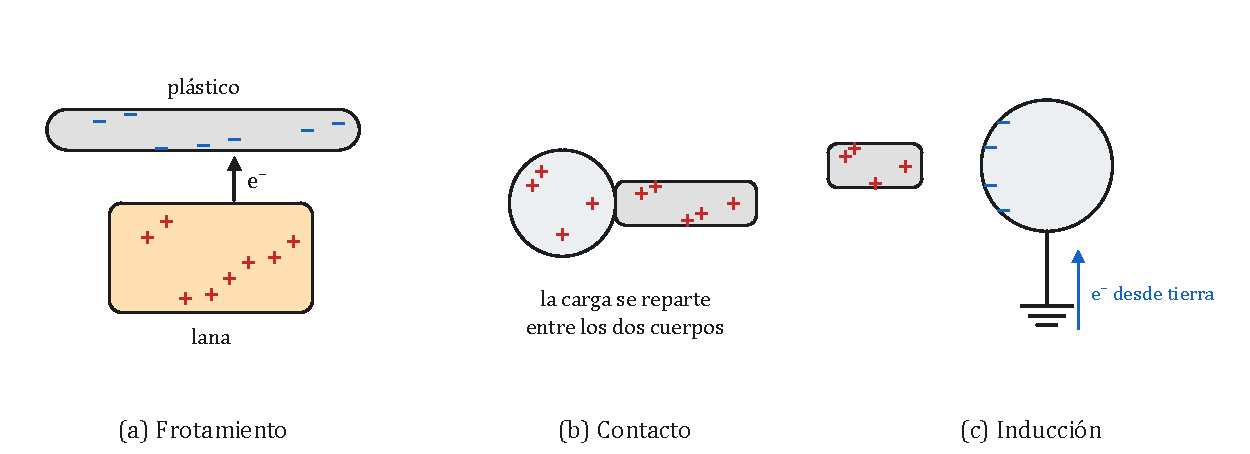
\includegraphics[width=0.95\linewidth]{images/UD5/electrizacion}
    \caption{Las tres formas de electrizar un cuerpo. En todas ellas solo se mueven electrones.}
    \label{fig:ele-electrizacion}
\end{figure}

\section{Ley de Coulomb}\label{sec:ele-coulomb}

En 1785 Charles-Augustin de Coulomb midió con una balanza de torsión la fuerza entre dos esferas cargadas.

\begin{definition}[Ley de Coulomb]
    La fuerza con que se atraen (si tienen signo contrario) o se repelen (si tienen el mismo signo) dos cargas puntuales es
    directamente proporcional al producto de las cargas e inversamente proporcional al cuadrado de la distancia que las separa:
    \begin{centeredequation}
        \boxed{\vec F = k\,\dfrac{Q\,q}{r^2}\,\vec u_r} \qquad\qquad F = k\,\dfrac{|Q|\,|q|}{r^2} \label{eq:ele-coulomb}
    \end{centeredequation}
    donde \(\vec u_r\) es un vector unitario que va de la carga que ejerce la fuerza a la que la sufre.
\end{definition}

Con los signos de las cargas incluidos, si \(Qq > 0\) la fuerza tiene el sentido de \(\vec u_r\) (repulsión) y si \(Qq < 0\),
el contrario (atracción) (figura~\ref{fig:ele-coulomb}).

\begin{figure}[H]
    \centering
    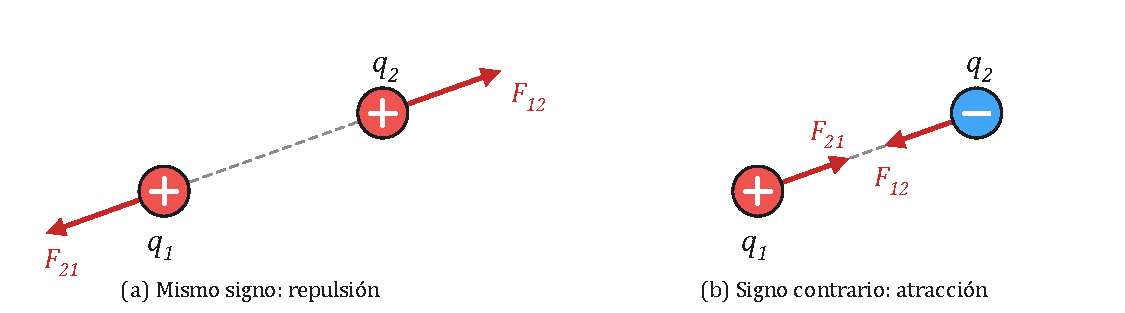
\includegraphics[width=0.8\linewidth]{images/UD5/coulomb}
    \caption{Las fuerzas entre dos cargas son iguales en módulo y de sentidos opuestos (tercera ley de Newton).}
    \label{fig:ele-coulomb}
\end{figure}

La constante \(k\) depende del medio. Se escribe \(k = \dfrac{1}{4\pi\varepsilon}\), donde \(\varepsilon\) es la
\azuln{permitividad} del medio. En el vacío:
\begin{centeredequation}
    \varepsilon_0 = \qty{8.85e-12}{\coulomb\squared\per\newton\per\m\squared} \qquad\qquad k = \dfrac{1}{4\pi\varepsilon_0} = \qty{8.99e9}{\newton\m\squared\per\coulomb\squared} \approx \qty{9e9}{\newton\m\squared\per\coulomb\squared}
\end{centeredequation}
En cualquier otro medio la permitividad es mayor y la fuerza, menor: el agua, por ejemplo, reduce la fuerza unas 80 veces
(por eso disuelve tan bien los compuestos iónicos).

\begin{remark}
    \textbf{Comparación con la gravedad.} Las dos leyes tienen la misma forma (inversamente proporcionales a \(r^2\)), pero:
    \begin{itemize}
        \item la fuerza gravitatoria siempre es atractiva; la eléctrica puede ser atractiva o repulsiva;
        \item \(G\) es universal; \(k\) depende del medio;
        \item la fuerza eléctrica es muchísimo más intensa: entre un protón y un electrón es unas \(10^{39}\) veces mayor que la
        gravitatoria. Si a gran escala domina la gravedad es porque los cuerpos grandes son prácticamente neutros.
    \end{itemize}
\end{remark}

\begin{exercise}
    ¿A qué distancia hay que poner dos cargas de \qty{2}{\micro\coulomb} para que se repelan con una fuerza de \qty{2}{\newton}?
    \begin{solu}
        \(r = \sqrt{\dfrac{k\,q^2}{F}} = \sqrt{\dfrac{9\cdot 10^9\cdot(2\cdot 10^{-6})^2}{2}} = \textcolor{red}{\qty{0.134}{\m} = \qty{13.4}{\cm}}\).
    \end{solu}
\end{exercise}

\begin{exercise}
    ¿Qué significado físico tiene la constante \(k\) de la ley de Coulomb?
    \begin{solu}
        \textcolor{blue}{Despejando, \(k = F r^2/(Qq)\).} \textcolor{red}{Es la fuerza con que se repelen dos cargas de
        \qty{1}{\coulomb} separadas \qty{1}{\m} en ese medio}: \textcolor{blue}{en el vacío, \qty{9e9}{\newton}, una fuerza enorme.}
    \end{solu}
\end{exercise}

\begin{exercise}
    Una partícula de \qty{50}{\g} con una carga de \qty{1}{\micro\coulomb} se mantiene en equilibrio \qty{30}{\cm} por encima
    de otra partícula fija, en su misma vertical. ¿Qué carga tiene la segunda partícula?
    \begin{solu}
        \textcolor{blue}{La fuerza eléctrica (repulsiva, hacia arriba) equilibra el peso: \(k\,\dfrac{q_1 q_2}{r^2} = mg\).}
        \[ q_2 = \dfrac{m g r^2}{k q_1} = \dfrac{0{,}05\cdot 9{,}8\cdot 0{,}3^2}{9\cdot 10^9\cdot 10^{-6}} = \textcolor{red}{\qty{4.9e-6}{\coulomb}} \]
        \textcolor{red}{Positiva}, \textcolor{blue}{para que haya repulsión.}
    \end{solu}
\end{exercise}

\paragraph{Principio de superposición.} Si sobre una carga actúan varias, la fuerza total es la suma vectorial de las fuerzas
que ejerce cada una: \(\vec F = \vec F_1 + \vec F_2 + \cdots\) Para calcularla: se ponen los ejes con el origen en la carga, se
calcula el módulo de cada fuerza, se dibuja su sentido (atracción o repulsión), se descompone en componentes y se suma.

\begin{exercise}
    Tres cargas de \qty{-3}{\micro\coulomb}, \qty{4}{\micro\coulomb} y \qty{2}{\micro\coulomb} están en los puntos \((3, 0)\),
    \((0, 4)\) y \((0, 0)\), con las coordenadas en centímetros. Calcula la fuerza sobre la tercera carga.
    \begin{solu}
        \textcolor{blue}{La de \qty{-3}{\micro\coulomb} atrae a la del origen hacia \(+X\); la de \qty{4}{\micro\coulomb} la repele hacia \(-Y\):}
        \[ F_1 = 9\cdot 10^9\,\dfrac{3\cdot 10^{-6}\cdot 2\cdot 10^{-6}}{0{,}03^2} = \qty{60}{\newton} \qquad F_2 = 9\cdot 10^9\,\dfrac{4\cdot 10^{-6}\cdot 2\cdot 10^{-6}}{0{,}04^2} = \qty{45}{\newton} \]
        \(\textcolor{red}{\vec F = 60\,\vec{i} - 45\,\vec{j}\ \unit{\newton}}\); \(F = \textcolor{red}{\qty{75}{\newton}}\).
    \end{solu}
\end{exercise}

\section{El campo eléctrico}\label{sec:ele-campo}

Una carga modifica el espacio que la rodea: crea un \rojon{campo eléctrico}. Otra carga colocada en él experimenta una fuerza.

\begin{definition}[Intensidad del campo eléctrico]
    La \rojon{intensidad del campo eléctrico} en un punto es la fuerza que actuaría sobre la unidad de carga positiva colocada
    en él: \(\vec E = \vec F/q\). Para el campo creado por una carga puntual \(Q\) a una distancia \(r\):
    \begin{centeredequation}
        \boxed{\vec E = k\,\dfrac{Q}{r^2}\,\vec u_r} \qquad\qquad E = k\,\dfrac{|Q|}{r^2} \label{eq:ele-E}
    \end{centeredequation}
    Se mide en \unit{\newton\per\coulomb}. Si \(Q > 0\), el campo se aleja de la carga; si \(Q < 0\), se dirige hacia ella.
\end{definition}

Conocido el campo, la fuerza sobre una carga \(q\) es \(\vec F = q\,\vec E\): sobre una carga positiva tiene el sentido del
campo, y sobre una negativa, el contrario. El campo creado por varias cargas es la suma vectorial de los campos de cada una
(\azuln{principio de superposición}).

\begin{exercise}
    Dos cargas de \qty{2e-8}{\coulomb} están en los puntos \((3, 0)\) y \((-3, 0)\) (en centímetros).
    \begin{enumerate}[label=\letraminuscula]
        \item Calcula el campo en el punto \((-6, 0)\) si las dos son positivas.
        \item Calcula el campo en el punto \((0, 3)\) si la de \((3, 0)\) es positiva y la de \((-3, 0)\), negativa.
    \end{enumerate}
    \begin{solu}
        \begin{enumerate}[label=\letraminuscula]
            \item \textcolor{blue}{Las dos están a la derecha del punto, a \qty{9}{\cm} y \qty{3}{\cm}; sus campos apuntan hacia \(-X\):}
            \(E_1 = 9\cdot 10^9\,\dfrac{2\cdot 10^{-8}}{0{,}09^2} = \qty{2.22e4}{\newton\per\coulomb}\);
            \(E_2 = \dfrac{9\cdot 10^9\cdot 2\cdot 10^{-8}}{0{,}03^2} = \qty{2e5}{\newton\per\coulomb}\).
            \(\textcolor{red}{\vec E = -2{,}22\cdot 10^5\,\vec{i}\ \unit{\newton\per\coulomb}}\).
            \item \textcolor{blue}{Las dos están a \(\sqrt{18}\ \unit{\cm}\): cada campo vale \(E = \qty{1e5}{\newton\per\coulomb}\). El de la
            positiva se aleja de ella, dirección \((-1, 1)/\sqrt 2\); el de la negativa va hacia ella, \((-1, -1)/\sqrt 2\). Las
            componentes \(y\) se anulan:}
            \(\textcolor{red}{\vec E = -2E\cos\ang{45}\,\vec{i} = -1{,}41\cdot 10^5\,\vec{i}\ \unit{\newton\per\coulomb}}\).
        \end{enumerate}
    \end{solu}
\end{exercise}

\subsection{Líneas del campo eléctrico}\label{subsec:ele-lineas}

Las líneas del campo eléctrico son tangentes en cada punto al vector \(\vec E\). \textbf{Salen de las cargas positivas}
(fuentes) y \textbf{llegan a las negativas} (sumideros); su número es proporcional a la carga y nunca se cortan
(figura~\ref{fig:ele-lineas}). Indican la trayectoria que seguiría una carga positiva muy pequeña abandonada en reposo solo
al principio de su movimiento, porque después la velocidad ya no tiene por qué seguir la línea.

\begin{figure}[H]
    \centering
    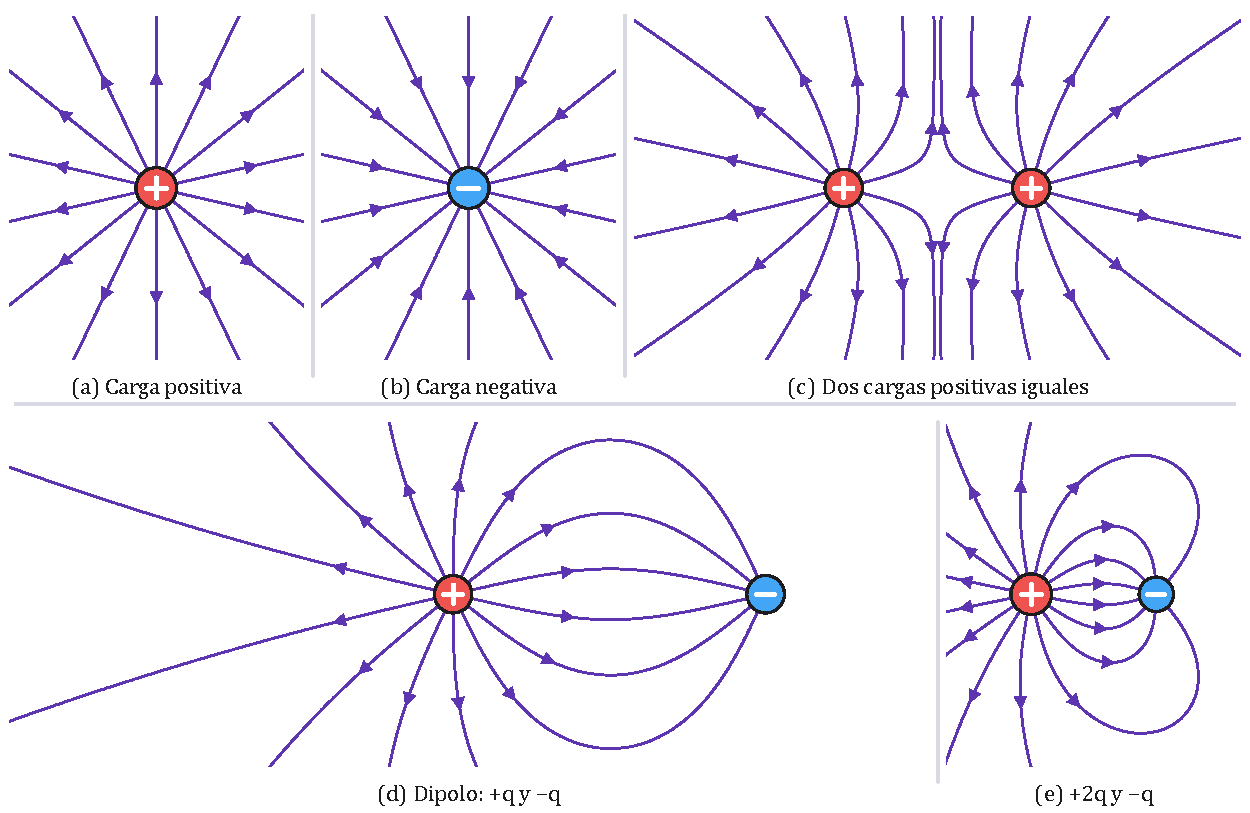
\includegraphics[width=0.95\linewidth]{images/UD5/lineas_campo}
    \caption{Líneas del campo eléctrico calculadas con la ley de Coulomb. Entre dos cargas iguales hay un punto en el que el
    campo es nulo; en (e), de la carga \(+2q\) salen el doble de líneas de las que llegan a \(-q\), y la mitad se van al infinito.}
    \label{fig:ele-lineas}
\end{figure}

\section{Energía potencial eléctrica}\label{sec:ele-energia}

La fuerza eléctrica es central y, como la gravitatoria, \textbf{conservativa}. Repitiendo el cálculo de la unidad anterior, el
trabajo que hace el campo de una carga \(Q\) sobre otra \(q\) que va de \(A\) a \(B\) es:
\begin{equation*}
    W_{A\to B} = \int_{r_A}^{r_B} k\,\dfrac{Q q}{r^2}\,dr = k\,\dfrac{Q q}{r_A} - k\,\dfrac{Q q}{r_B} = E_{p,A} - E_{p,B}
\end{equation*}
Tomando \(E_p = 0\) en el infinito, la \rojon{energía potencial eléctrica} de dos cargas separadas una distancia \(r\) es:
\begin{centeredequation}
    \boxed{E_p = k\,\dfrac{Q\,q}{r}} \label{eq:ele-ep}
\end{centeredequation}
Ahora los signos de las cargas importan: \(E_p\) es \textbf{positiva} si las cargas tienen el mismo signo (se repelen) y
\textbf{negativa} si tienen signos contrarios (se atraen). Los procesos espontáneos (el campo hace trabajo positivo) son los
que disminuyen la energía potencial: separar cargas del mismo signo o acercar cargas de signo contrario.

Si hay más de dos cargas, la energía potencial del sistema es la suma de las energías de cada pareja:
\(E_p = k\left(\dfrac{q_1 q_2}{r_{12}} + \dfrac{q_1 q_3}{r_{13}} + \dfrac{q_2 q_3}{r_{23}}\right)\).

\begin{exercise}
    En los vértices de un triángulo equilátero de \qty{30}{\cm} de lado hay cargas de \qty{3}{\micro\coulomb},
    \qty{-6}{\micro\coulomb} y \qty{-9}{\micro\coulomb}. Calcula la energía potencial del sistema.
    \begin{solu}
        \[ E_p = \dfrac{k}{r}\,(q_1q_2 + q_1q_3 + q_2q_3) = \dfrac{9\cdot 10^9}{0{,}3}\,(-18 - 27 + 54)\cdot 10^{-12} = \textcolor{red}{\qty{0.27}{\joule}} \]
    \end{solu}
\end{exercise}

\section{Potencial eléctrico}\label{sec:ele-potencial}

\begin{definition}[Potencial eléctrico]
    El \rojon{potencial eléctrico} en un punto es la energía potencial por unidad de carga positiva colocada en él,
    \(V = E_p/q\). Para una carga puntual \(Q\):
    \begin{centeredequation}
        \boxed{V = k\,\dfrac{Q}{r}} \label{eq:ele-V}
    \end{centeredequation}
    Es un escalar y se mide en \azuln{voltios}: \(\qty{1}{\volt} = \qty{1}{\joule\per\coulomb}\). Es positivo cerca de las cargas
    positivas y negativo cerca de las negativas, y vale cero en el infinito.
\end{definition}

El potencial creado por varias cargas es la \textbf{suma algebraica} de los potenciales de cada una (con su signo):
\(V = V_1 + V_2 + \cdots\) Es mucho más fácil de calcular que el campo, porque no hay que sumar vectores.

\paragraph{Trabajo y diferencia de potencial.} El trabajo que hace el campo al llevar una carga \(q\) de \(A\) a \(B\) es:
\begin{centeredequation}
    \boxed{W_{A\to B} = -\Delta E_p = q\,(V_A - V_B)} \label{eq:ele-trabajo}
\end{centeredequation}
El trabajo que hay que hacer con un agente externo para llevarla (sin que gane energía cinética) es el opuesto. Una carga
positiva abandonada a sí misma se mueve espontáneamente hacia potenciales \textbf{menores}; una negativa, hacia potenciales
\textbf{mayores}. En los dos casos disminuye su energía potencial.

\begin{exercise}
    Tres cargas de \qty{-2}{\micro\coulomb}, \qty{-8}{\micro\coulomb} y \qty{6}{\micro\coulomb} están en los puntos \((4, 0)\),
    \((0, 0)\) y \((0, 3)\) (en metros). Calcula el potencial en el punto \((4, 3)\).
    \begin{solu}
        \textcolor{blue}{Distancias al punto: \qty{3}{\m}, \qty{5}{\m} y \qty{4}{\m}.}
        \[ V = 9\cdot 10^9\left(\dfrac{-2}{3} + \dfrac{-8}{5} + \dfrac{6}{4}\right)\cdot 10^{-6} = \textcolor{red}{\qty{-6900}{\volt}} \]
    \end{solu}
\end{exercise}

\begin{exercise}
    Dos cargas de \qty{3}{\micro\coulomb} y \qty{-5}{\micro\coulomb} están en \((0, 4)\) y \((0, -4)\) (en metros). ¿Qué trabajo hace
    el campo al llevar una carga de \qty{2}{\micro\coulomb} desde el origen hasta el punto \((3, 0)\)? ¿Y un agente externo?
    \begin{solu}
        \(V_A = 9\cdot 10^9\,\dfrac{(3 - 5)\cdot 10^{-6}}{4} = \qty{-4500}{\volt}\);
        \(V_B = 9\cdot 10^9\,\dfrac{(3 - 5)\cdot 10^{-6}}{5} = \qty{-3600}{\volt}\).

        \(W_{\text{campo}} = q(V_A - V_B) = 2\cdot 10^{-6}\cdot(-900) = \textcolor{red}{\qty{-1.8e-3}{\joule}}\);
        \(W_{\text{ext}} = \textcolor{red}{\qty{1.8e-3}{\joule}}\). \textcolor{blue}{Hay que forzar a la carga positiva a ir hacia potenciales mayores.}
    \end{solu}
\end{exercise}

\subsection{Relación entre el campo y el potencial}\label{subsec:ele-E-V}

De \(W = -q\,\Delta V\) y \(dW = q\,\vec E\cdot d\vec r\) se obtiene \(dV = -\vec E\cdot d\vec r\). En una dirección \(x\):
\begin{centeredequation}
    E_x = -\,\dfrac{dV}{dx} \label{eq:ele-E-dV}
\end{centeredequation}
\textbf{El campo apunta siempre hacia los potenciales decrecientes}, y es más intenso donde el potencial cambia más deprisa.

\paragraph{Superficies equipotenciales.} Son los lugares de igual potencial; para una carga puntual, esferas centradas en
ella. Como sobre una equipotencial \(dV = 0\), \(\vec E\cdot d\vec r = 0\): \textbf{las líneas de campo son perpendiculares a
las superficies equipotenciales}, y mover una carga sobre una de ellas no cuesta trabajo (figura~\ref{fig:ele-dipolo}).

\begin{figure}[H]
    \centering
    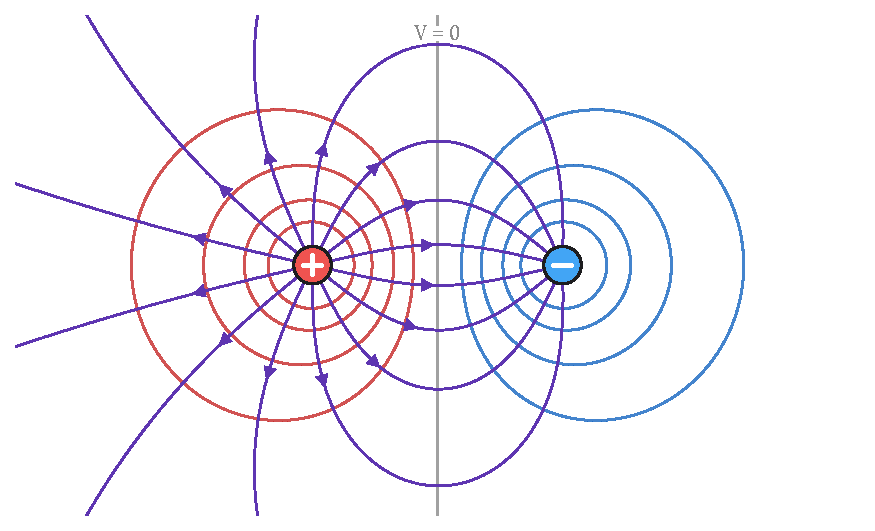
\includegraphics[width=0.66\linewidth]{images/UD5/dipolo}
    \caption{Equipotenciales (positivas en rojo, negativas en azul, \(V = 0\) en gris) y líneas de campo (morado) de un dipolo.
    Se cortan siempre en ángulo recto.}
    \label{fig:ele-dipolo}
\end{figure}

\subsection{Campo uniforme entre placas paralelas}\label{subsec:ele-placas}

Entre dos placas planas paralelas con cargas opuestas el campo es \textbf{uniforme}: tiene el mismo valor en todos los puntos,
va de la placa positiva a la negativa y las equipotenciales son planos paralelos a las placas (figura~\ref{fig:ele-placas}).
Integrando \(dV = -E\,dx\) con \(E\) constante:
\begin{centeredequation}
    \boxed{V_A - V_B = E\,d} \qquad\Rightarrow\qquad E = \dfrac{\Delta V}{d} \label{eq:ele-placas}
\end{centeredequation}
Por eso el campo eléctrico también se mide en \unit{\volt\per\m} (\(\qty{1}{\volt\per\m} = \qty{1}{\newton\per\coulomb}\)).

\begin{figure}[H]
    \centering
    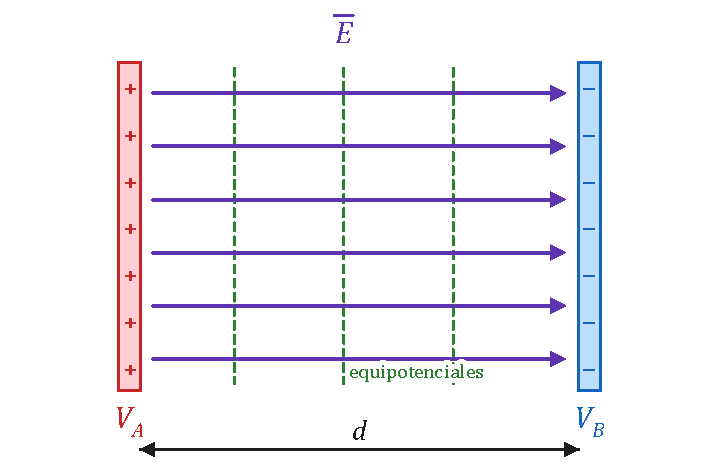
\includegraphics[width=0.5\linewidth]{images/UD5/placas}
    \caption{Campo uniforme entre dos placas paralelas.}
    \label{fig:ele-placas}
\end{figure}

\begin{exercise}
    Dos placas paralelas separadas \qty{5}{\cm} tienen una diferencia de potencial de \qty{6000}{\volt}. Se libera un protón en
    reposo junto a la placa positiva. Calcula el campo entre las placas y la velocidad con que llega el protón a la negativa
    (\(q_p = \qty{1.6e-19}{\coulomb}\), \(m_p = \qty{1.67e-27}{\kg}\)).
    \begin{solu}
        \(E = \dfrac{\Delta V}{d} = \dfrac{6000}{0{,}05} = \textcolor{red}{\qty{1.2e5}{\newton\per\coulomb}}\).

        \textcolor{blue}{El trabajo del campo se convierte en energía cinética: \(q\,\Delta V = \tfrac{1}{2}m v^2\).}
        \(v = \sqrt{\dfrac{2 q\,\Delta V}{m}} = \sqrt{\dfrac{2\cdot 1{,}6\cdot 10^{-19}\cdot 6000}{1{,}67\cdot 10^{-27}}} = \textcolor{red}{\qty{1.07e6}{\m\per\second}}\).
    \end{solu}
\end{exercise}

\subsection{Movimiento de cargas en un campo uniforme}\label{subsec:ele-movimiento}

Sobre una carga en un campo uniforme actúa una fuerza constante \(\vec F = q\vec E\), y su aceleración es \(\vec a = q\vec E/m\):
el problema es igual que el de un tiro en el campo gravitatorio, pero con otra «gravedad». Si una partícula entra con velocidad
\(\vec v_0\) perpendicular al campo, su movimiento es uniforme en la dirección de \(\vec v_0\) y uniformemente acelerado en la
del campo, y describe una \textbf{parábola} (figura~\ref{fig:ele-desviacion}). En esto se basaban los tubos de rayos catódicos de
los televisores antiguos, y se basan las impresoras de chorro de tinta.

\begin{figure}[H]
    \centering
    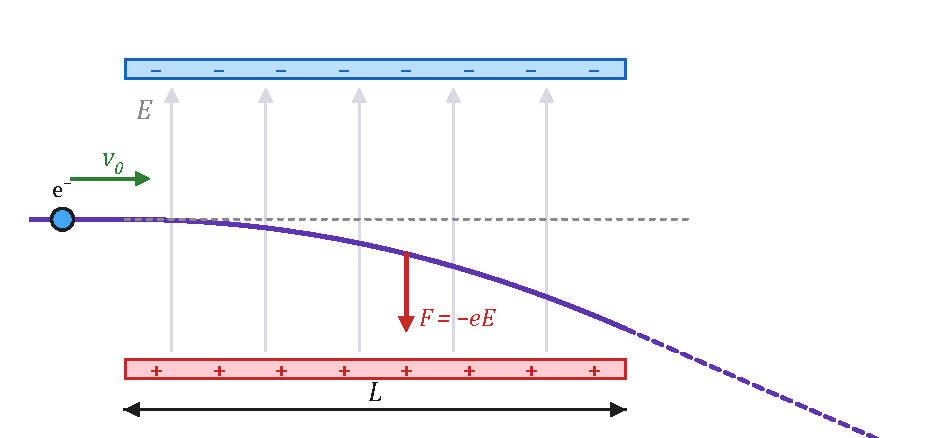
\includegraphics[width=0.66\linewidth]{images/UD5/desviacion}
    \caption{Un electrón que entra horizontalmente en un campo vertical se desvía en sentido contrario al campo.}
    \label{fig:ele-desviacion}
\end{figure}

\begin{exercise}
    Si una carga positiva se mueve en sentido contrario al campo, ¿aumenta o disminuye su energía potencial? ¿Y si es negativa?
    \begin{solu}
        \textcolor{blue}{Al ir en contra del campo va hacia potenciales mayores (\(\Delta V > 0\)), y \(\Delta E_p = q\,\Delta V\).}
        \textcolor{red}{Si es positiva, su energía potencial aumenta} (hay que empujarla); \textcolor{red}{si es negativa, disminuye}
        (ese movimiento es espontáneo para ella).
    \end{solu}
\end{exercise}

\section{Flujo eléctrico y teorema de Gauss}\label{sec:ele-gauss}

\subsection{Flujo del campo eléctrico}\label{subsec:ele-flujo}

El \rojon{flujo} del campo eléctrico a través de una superficie mide el número de líneas de campo que la atraviesan.
Representamos la superficie con un vector \(\vec S\) perpendicular a ella, de módulo igual a su área. Para un campo uniforme y
una superficie plana:
\begin{centeredequation}
    \boxed{\Phi = \vec E\cdot\vec S = E\,S\cos\alpha} \label{eq:ele-flujo}
\end{centeredequation}
El flujo es máximo si la superficie es perpendicular a las líneas (\(\alpha = 0\)) y nulo si es paralela a ellas. Se mide en
\unit{\newton\m\squared\per\coulomb}. Si el campo no es uniforme o la superficie es curva, se divide en elementos \(d\vec S\) y se
suma: \(\Phi = \oint\vec E\cdot d\vec S\). En una superficie cerrada, \(d\vec S\) apunta hacia fuera, así que las líneas que
salen cuentan como flujo positivo y las que entran, como negativo.

\begin{figure}[H]
    \centering
    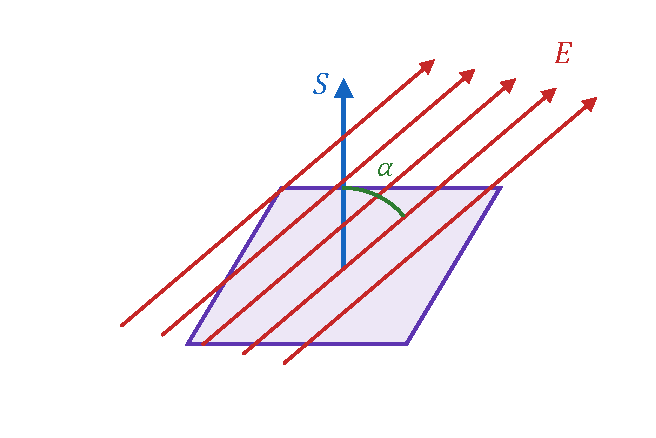
\includegraphics[width=0.45\linewidth]{images/UD5/flujo}
    \caption{El flujo depende del campo, del área y del ángulo \(\alpha\) entre \(\vec E\) y \(\vec S\).}
    \label{fig:ele-flujo}
\end{figure}

\subsection{Teorema de Gauss}\label{subsec:ele-teorema-gauss}

Calculemos el flujo del campo de una carga \(Q\) a través de una esfera de radio \(r\) centrada en ella (una \azuln{superficie
gaussiana}). En cada punto \(\vec E\) es radial, paralelo a \(d\vec S\), y vale \(kQ/r^2\):
\begin{equation*}
    \Phi = \oint E\,dS = \dfrac{kQ}{r^2}\oint dS = \dfrac{kQ}{r^2}\,4\pi r^2 = 4\pi k Q = \dfrac{Q}{\varepsilon_0}
\end{equation*}
El resultado no depende del radio, y como el número de líneas que atraviesan cualquier otra superficie cerrada que rodee la
carga es el mismo, vale para cualquier forma. Sumando para varias cargas:

\begin{definition}[Teorema de Gauss]
    El flujo eléctrico a través de cualquier superficie cerrada es igual a la carga neta encerrada en su interior dividida por
    la permitividad del vacío:
    \begin{centeredequation}
        \boxed{\Phi = \oint\vec E\cdot d\vec S = \dfrac{Q_{\text{int}}}{\varepsilon_0}} \label{eq:ele-gauss}
    \end{centeredequation}
    Las cargas exteriores no contribuyen: sus líneas entran y salen, y su flujo neto es nulo.
\end{definition}

\begin{figure}[H]
    \centering
    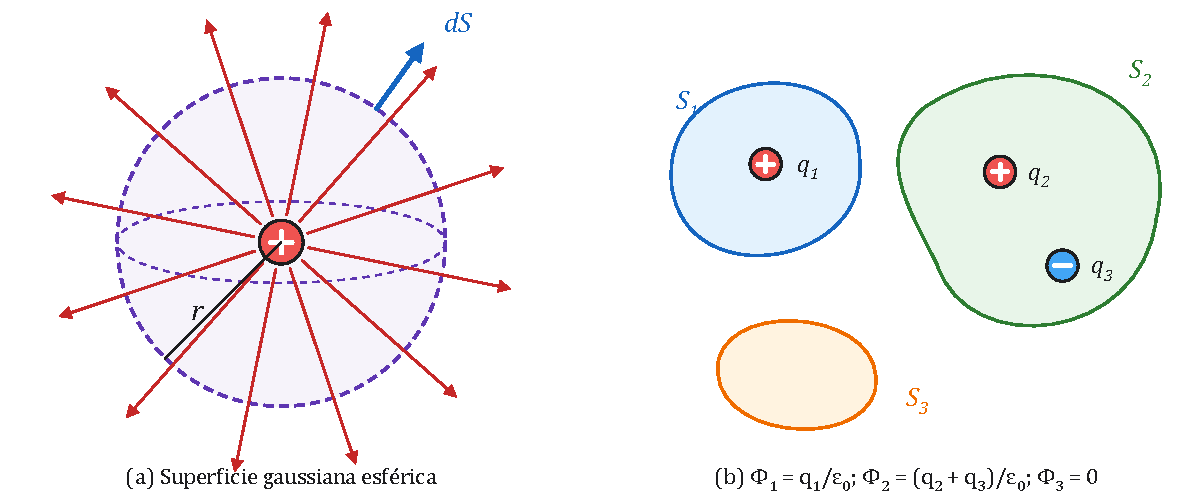
\includegraphics[width=0.95\linewidth]{images/UD5/gauss}
    \caption{(a) Esfera gaussiana alrededor de una carga. (b) El flujo a través de cada superficie cerrada solo depende de la
    carga encerrada.}
    \label{fig:ele-gauss}
\end{figure}

\subsection{Aplicaciones del teorema de Gauss}\label{subsec:ele-aplicaciones}

El teorema de Gauss permite calcular de forma muy sencilla el campo de distribuciones de carga simétricas. Se elige una
superficie gaussiana en la que el campo sea perpendicular a ella y tenga el mismo valor en todos sus puntos (o sea paralelo,
y no aporte flujo).

\paragraph{a) Conductor en equilibrio.} Dentro de un conductor en equilibrio el campo es nulo: si no lo fuera, las cargas
libres se moverían. Por el teorema de Gauss, la carga encerrada por cualquier superficie interior es nula: \textbf{toda la carga
de un conductor se reparte por su superficie}. Además, fuera del conductor el campo es perpendicular a la superficie (si
tuviera una componente paralela, movería las cargas), y todo el conductor está al mismo potencial. Por eso un coche o un
avión son buenos refugios frente a un rayo (\emph{jaula de Faraday}).

\paragraph{b) Esfera cargada.} Fuera de una esfera de radio \(R\) con carga \(Q\), cogiendo una superficie gaussiana esférica
de radio \(r > R\): \(E\cdot 4\pi r^2 = Q/\varepsilon_0\), es decir,
\begin{centeredequation}
    E = k\,\dfrac{Q}{r^2} \qquad (r \geq R) \label{eq:ele-esfera-fuera}
\end{centeredequation}
\textbf{Fuera de ella, una esfera cargada crea el mismo campo que una carga puntual en su centro.} Dentro hay que distinguir:
\begin{itemize}
    \item \emph{Esfera conductora} (o hueca, con la carga en la superficie): la carga encerrada es nula y \(E = 0\) para \(r < R\).
    \item \emph{Esfera maciza aislante con carga uniforme} de densidad \(\rho = Q/\tfrac{4}{3}\pi R^3\): la carga encerrada es
    \(Q\,r^3/R^3\), y queda
    \begin{centeredequation}
        E = k\,\dfrac{Q\,r}{R^3} \qquad (r \leq R) \label{eq:ele-esfera-dentro}
    \end{centeredequation}
    el campo crece linealmente desde el centro, igual que el gravitatorio dentro de la Tierra.
\end{itemize}

\paragraph{c) Hilo indefinido.} Para un hilo recto con densidad lineal de carga \(\lambda = q/L\) se toma un cilindro coaxial
de radio \(r\) y altura \(h\). En las bases el campo es paralelo a la superficie y no hay flujo; en la superficie lateral es
perpendicular y constante (figura~\ref{fig:ele-gauss-aplicaciones}a):
\begin{equation*}
    E\cdot 2\pi r h = \dfrac{\lambda h}{\varepsilon_0} \qquad\Rightarrow\qquad \boxed{E = \dfrac{\lambda}{2\pi\varepsilon_0\,r}}
\end{equation*}

\paragraph{d) Plano indefinido.} Para un plano con densidad superficial de carga \(\sigma = Q/S\), se toma un cilindro que lo
atraviesa. Solo hay flujo por las dos bases (figura~\ref{fig:ele-gauss-aplicaciones}b):
\begin{equation*}
    2\,E\,S = \dfrac{\sigma S}{\varepsilon_0} \qquad\Rightarrow\qquad \boxed{E = \dfrac{\sigma}{2\varepsilon_0}}
\end{equation*}
El campo no depende de la distancia al plano. Entre dos placas paralelas con cargas \(+\sigma\) y \(-\sigma\), los campos de
las dos se suman entre ellas y se anulan fuera: \(E = \sigma/\varepsilon_0\), el campo uniforme del apartado anterior.

\begin{figure}[H]
    \centering
    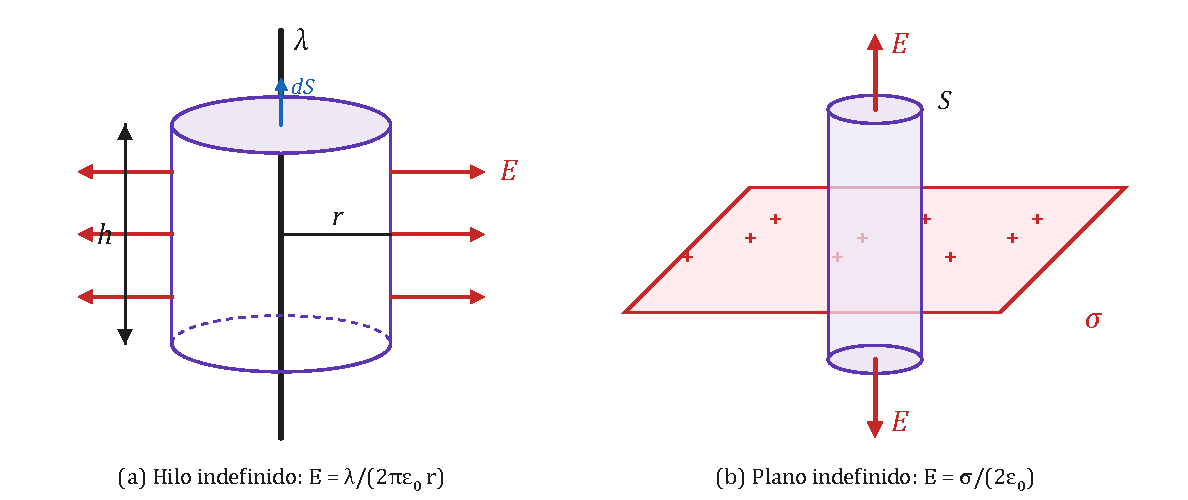
\includegraphics[width=0.95\linewidth]{images/UD5/gauss_aplicaciones}
    \caption{Superficies gaussianas para un hilo y para un plano cargados.}
    \label{fig:ele-gauss-aplicaciones}
\end{figure}

\begin{exercise}
    Una esfera maciza aislante de \qty{15}{\cm} de radio tiene una carga de \qty{6}{\micro\coulomb} repartida uniformemente.
    Calcula, con el teorema de Gauss, el campo a \qty{5}{\cm} y a \qty{20}{\cm} de su centro.
    \begin{solu}
        \(r = \qty{0.05}{\m}\) (dentro): \(E = k\,\dfrac{Q r}{R^3} = 9\cdot 10^9\,\dfrac{6\cdot 10^{-6}\cdot 0{,}05}{0{,}15^3} = \textcolor{red}{\qty{8.0e5}{\newton\per\coulomb}}\).

        \(r = \qty{0.20}{\m}\) (fuera): \(E = k\,\dfrac{Q}{r^2} = \textcolor{red}{\qty{1.35e6}{\newton\per\coulomb}}\).
    \end{solu}
\end{exercise}

\begin{exercise}
    Una esfera hueca conductora de \qty{25}{\cm} de radio tiene una carga de \qty{8}{\micro\coulomb}. Calcula el campo a
    \qty{12}{\cm} y a \qty{40}{\cm} de su centro.
    \begin{solu}
        \textcolor{red}{A \qty{12}{\cm}, \(E = 0\)}: \textcolor{blue}{no hay carga encerrada.}
        A \qty{40}{\cm}: \(E = 9\cdot 10^9\,\dfrac{8\cdot 10^{-6}}{0{,}4^2} = \textcolor{red}{\qty{4.5e5}{\newton\per\coulomb}}\).
    \end{solu}
\end{exercise}

\begin{exercise}
    Un hilo muy largo tiene una carga de \qty{2}{\micro\coulomb} por metro. ¿Cuánto vale el campo a \qty{30}{\cm} de él? ¿Y el
    de una lámina plana muy grande con \qty{5}{\micro\coulomb\per\m\squared}?
    \begin{solu}
        \(E_{\text{hilo}} = \dfrac{\lambda}{2\pi\varepsilon_0 r} = \dfrac{2\cdot 10^{-6}}{2\pi\cdot 8{,}85\cdot 10^{-12}\cdot 0{,}3} = \textcolor{red}{\qty{1.20e5}{\newton\per\coulomb}}\).

        \(E_{\text{plano}} = \dfrac{\sigma}{2\varepsilon_0} = \dfrac{5\cdot 10^{-6}}{2\cdot 8{,}85\cdot 10^{-12}} = \textcolor{red}{\qty{2.82e5}{\newton\per\coulomb}}\), \textcolor{blue}{a cualquier distancia.}
    \end{solu}
\end{exercise}

\section{Esferas conductoras unidas por un hilo}\label{sec:ele-esferas}

El potencial de una esfera conductora de radio \(r\) y carga \(q\) es el de su superficie, \(V = kq/r\). Si se unen dos esferas
con un hilo conductor, pasan cargas de la de mayor potencial a la de menor hasta que los potenciales se igualan
(figura~\ref{fig:ele-esferas}). Las condiciones son:
\begin{centeredequation}
    \text{igualdad de potenciales: } \dfrac{k\,q'_1}{r_1} = \dfrac{k\,q'_2}{r_2} \qquad\qquad \text{conservación de la carga: } q'_1 + q'_2 = q_1 + q_2 \label{eq:ele-esferas}
\end{centeredequation}
La carga final de cada esfera es proporcional a su radio: la esfera grande se queda con más carga, pero la densidad de carga
es mayor en la pequeña. Por eso el campo es más intenso en las zonas puntiagudas de un conductor (\emph{efecto de las puntas},
en el que se basan los pararrayos).

\begin{figure}[H]
    \centering
    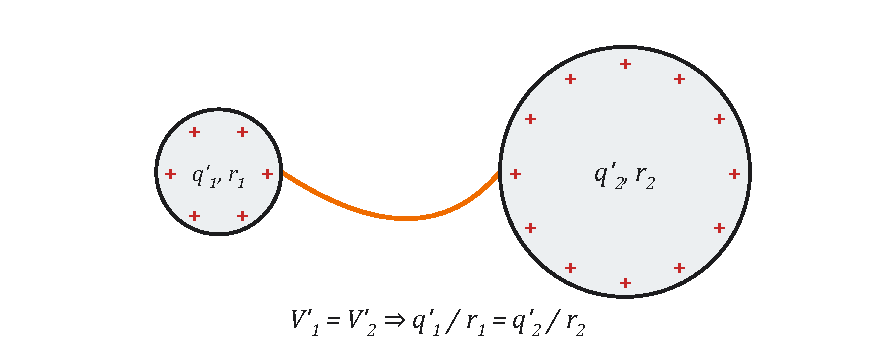
\includegraphics[width=0.62\linewidth]{images/UD5/esferas_hilo}
    \caption{Al unirlas, las dos esferas quedan al mismo potencial.}
    \label{fig:ele-esferas}
\end{figure}

\begin{exercise}
    Dos esferas metálicas de \qty{3}{\cm} y \qty{6}{\cm} de radio tienen cada una una carga de \qty{4e-8}{\coulomb}. Si se unen
    con un hilo conductor, ¿qué carga y qué potencial tendrá cada una?
    \begin{solu}
        \textcolor{blue}{\(q'_1 + q'_2 = \qty{8e-8}{\coulomb}\) y \(q'_1/0{,}03 = q'_2/0{,}06 \Rightarrow q'_2 = 2q'_1\).}
        \(q'_1 = \textcolor{red}{\qty{2.67e-8}{\coulomb}}\); \(q'_2 = \textcolor{red}{\qty{5.33e-8}{\coulomb}}\);
        \(V = 9\cdot 10^9\,\dfrac{2{,}67\cdot 10^{-8}}{0{,}03} = \textcolor{red}{\qty{8000}{\volt}}\) \textcolor{blue}{(las dos).}
    \end{solu}
\end{exercise}

\section{Resumen de fórmulas}\label{sec:ele-resumen}

\begin{table}[H]
    \centering
    \caption{Fórmulas principales del campo eléctrico}
    \vspace{-5pt}
    \begin{tabular}{@{}lL{10cm}@{}}
        \toprule
        \textbf{Magnitud} & \textbf{Expresión} \\
        \midrule
        Ley de Coulomb & \(F = k\,|Q q|/r^2\), \quad \(k = 1/(4\pi\varepsilon_0) = \qty{9e9}{\newton\m\squared\per\coulomb\squared}\) \\[3pt]
        Campo eléctrico & \(E = k\,|Q|/r^2\), \quad \(\vec F = q\vec E\) \\[3pt]
        Energía potencial & \(E_p = kQq/r\) (con signos) \\[3pt]
        Potencial & \(V = kQ/r\), \quad \(V = \sum V_i\), \quad \(W_{A\to B} = q(V_A - V_B)\) \\[3pt]
        Campo y potencial & \(E_x = -dV/dx\); \quad campo uniforme: \(V_A - V_B = E\,d\) \\[3pt]
        Flujo & \(\Phi = \vec E\cdot\vec S = E S\cos\alpha\) \\[3pt]
        Teorema de Gauss & \(\Phi = Q_{\text{int}}/\varepsilon_0\) \\[3pt]
        Esfera de carga \(Q\) & fuera: \(E = kQ/r^2\); \quad dentro: conductora \(E = 0\), maciza \(E = kQr/R^3\) \\[3pt]
        Hilo y plano & \(E = \lambda/(2\pi\varepsilon_0 r)\); \quad \(E = \sigma/(2\varepsilon_0)\) \\[3pt]
        Esferas unidas & \(q'_1/r_1 = q'_2/r_2\), \quad \(q'_1 + q'_2 = q_1 + q_2\) \\
        \bottomrule
    \end{tabular}
    \label{tab:ele-resumen}
\end{table}

\begin{table}[H]
    \centering
    \caption{Comparación entre el campo gravitatorio y el eléctrico}
    \vspace{-5pt}
    \begin{tabular}{@{}lL{5.4cm}L{5.4cm}@{}}
        \toprule
        & \textbf{Gravitatorio} & \textbf{Eléctrico} \\
        \midrule
        Lo crea & la masa & la carga \\[3pt]
        Fuerza & siempre atractiva & atractiva o repulsiva \\[3pt]
        Constante & \(G\), universal y muy pequeña & \(k\), depende del medio y es muy grande \\[3pt]
        Líneas de campo & solo llegan a las masas & salen de las cargas positivas y llegan a las negativas \\[3pt]
        Potencial & \(V = -GM/r\), siempre negativo & \(V = kQ/r\), con el signo de \(Q\) \\[3pt]
        En común & \multicolumn{2}{L{10.8cm}}{Fuerzas centrales, conservativas e inversamente proporcionales al cuadrado de la distancia} \\
        \bottomrule
    \end{tabular}
    \label{tab:ele-comparacion}
\end{table}

\section{Prácticas de laboratorio}\label{sec:ele-practicas}

\subsection{Práctica 1: superficies equipotenciales en una cubeta}\label{subsec:ele-practica-cubeta}

\noindent\begin{minipage}[t]{0.56\linewidth}
\textbf{Objetivo.} Localizar las líneas equipotenciales entre dos electrodos y dibujar a partir de ellas las líneas de campo.

\textbf{Material.} Cubeta de fondo plano con una capa de agua del grifo de 1 o 2 cm, papel milimetrado debajo, dos electrodos
(láminas metálicas o clavos gruesos), fuente de corriente continua de 6 a 12 V, voltímetro digital y cables.

\textbf{Procedimiento.}
\begin{enumerate}[label=\numberballmDarkTeal]
    \item Conecta los electrodos a la fuente y el terminal negativo del voltímetro al electrodo negativo
    (figura~\ref{fig:ele-practica}).
    \item Con la otra punta del voltímetro, busca varios puntos en los que marque, por ejemplo, \qty{3}{\volt} y anota sus
    coordenadas en el papel. Repite con \qty{6}{\volt} y \qty{9}{\volt}.
    \item Une los puntos de igual potencial y dibuja las líneas de campo perpendiculares a ellos.
    \item Repite con dos electrodos puntuales (clavos).
\end{enumerate}
\end{minipage}\hfill
\begin{minipage}[t]{0.4\linewidth}
    \vspace{0pt}
    \centering
    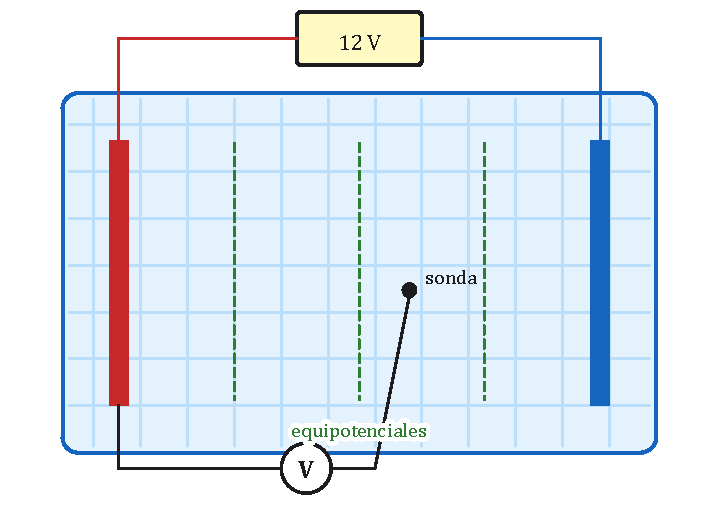
\includegraphics[width=\linewidth]{images/UD5/practica_equipotenciales}
    \captionof{figure}{Montaje con dos electrodos planos.}
    \label{fig:ele-practica}
\end{minipage}

\textbf{Cuestiones.}
\begin{enumerate}[label=\letraminuscula]
    \item Con los electrodos planos, ¿cómo son las equipotenciales? ¿Están igual de separadas? Calcula el campo con \(E = \Delta V/d\).
    \item Compara el mapa de los electrodos puntuales con la figura~\ref{fig:ele-dipolo}.
    \item ¿Por qué no circula apenas corriente por el voltímetro? ¿Por qué hay que usar agua del grifo y no agua destilada?
\end{enumerate}

\subsection{Práctica 2: el péndulo eléctrico}\label{subsec:ele-practica-pendulo}

\noindent\begin{minipage}[t]{0.6\linewidth}
\textbf{Objetivo.} Observar la electrización por frotamiento, contacto e inducción y estimar la carga de una bolita.

\textbf{Material.} Bolita de papel de aluminio (o de corcho blanco recubierta) colgada de un hilo de seda o de nailon de unos
\qty{30}{\cm}, varillas de plástico y de vidrio, paño de lana, balanza de precisión y regla.

\textbf{Procedimiento.}
\begin{enumerate}[label=\numberballmDarkTeal]
    \item Frota la varilla de plástico y acércala a la bolita sin tocarla: observa que la atrae (inducción).
    \item Deja que la toque: después la repele (contacto). Repite con la de vidrio y compara.
    \item Carga por contacto dos bolitas iguales colgadas del mismo punto y mide el ángulo que forman sus hilos en el equilibrio.
\end{enumerate}
\end{minipage}\hfill
\begin{minipage}[t]{0.36\linewidth}
    \vspace{0pt}
    \centering
    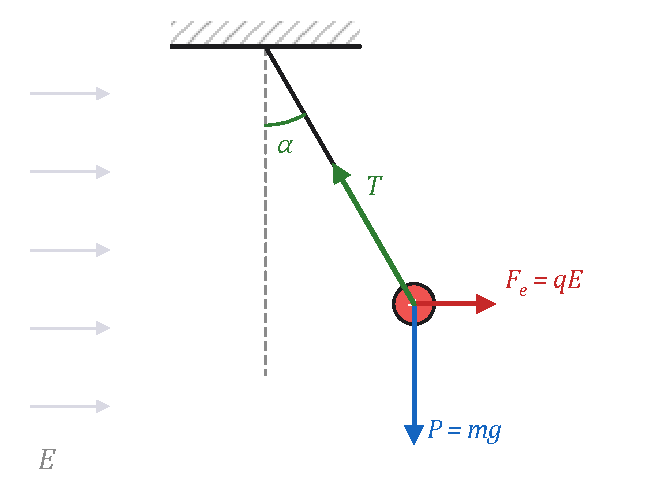
\includegraphics[width=\linewidth]{images/UD5/pendulo_electrico}
    \captionof{figure}{Fuerzas sobre una bolita cargada en equilibrio.}
    \label{fig:ele-pendulo}
\end{minipage}

\textbf{Cálculos.} En el equilibrio, \(T\cos\alpha = mg\) y \(T\sen\alpha = F_e\), así que \(F_e = mg\tg\alpha\). Con
\(F_e = k\,q^2/r^2\) y la separación \(r\) entre las bolitas, estima su carga.

\textbf{Cuestiones.}
\begin{enumerate}[label=\letraminuscula]
    \item ¿Por qué la bolita neutra es atraída por la varilla aunque no tenga carga neta?
    \item ¿Por qué la experiencia sale peor un día húmedo?
    \item ¿De qué orden es la carga obtenida? Exprésala en número de electrones.
\end{enumerate}
